\chapter{Avaliação quantitativa}\label{chap:avaliacao}

O objetivo deste capítulo é descrever as avaliações utilizadas na solução proposta. A avaliação tem como objetivo determinar a performance e o percentual de perdas do mecanismo de descoberta, conexão e desconexão de \smartobjs.

A avaliação será realizada por meio de experimentos, onde a performance será avaliada através da contagem de tempo desde que o \mhub efetivamente descobre um objeto até o momento em que a aplicação é informada sobre este evento. O percentual de perdas da solução consistirá na verificação de quantas operações de conexão, desconexão e descoberta geraram eventos correspondentes para a aplicação.

Em todos os experimentos, utilizou-se o \ubroker interno do \mhubcddl.

\section{Experimento 1}\label{chap:avaliacao-experimento1}


\subsection{Métricas}

A fim de determinar a performance da solução em relação à entrega dos eventos de descoberta, a aplicação permanece constantemente anotando os \timestamps de cada evento de descoberta emitido pelo \stwopa, e os \timestamps de notificações destes eventos na aplicação---ambos em milissegundos. O primeiro \timestamp é subtraído do segundo de forma a calcular o tempo de propagação dos eventos de descoberta, que será de agora em diante referido como $\Delta t_{descoberta}$ e calculado conforme a \autoref{equ:performance-discovery}.
\begin{equation}
	\label{equ:performance-discovery}
	\Delta t_{descoberta} = t_{descoberta,app} - t_{descoberta,\stwopa}
\end{equation}

Onde $t_{descoberta,app}$ e $t_{descoberta,\stwopa}$ se referem ao \timestamp de uma notificação de descoberta na aplicação e ao \timestamp do evento de descoberta gerado pelo \stwopa, respectivamente.

Na \autoref{img:performance-annotation} é possível observar onde os \timestamps utilizados na avaliação de performance são anotados. Ambos os \timestamps são denotados na imagem por um cronômetro. Na imagem, $T0$ e $T1$ são equivalentes à $t_{descoberta,\stwopa}$ e $t_{descoberta,app}$ da \autoref{equ:performance-discovery}.

\begin{figure}[htb]
	
	\begin{center}

		\caption{\label{img:performance-annotation}Componentes onde há a captura de \timestamps}
		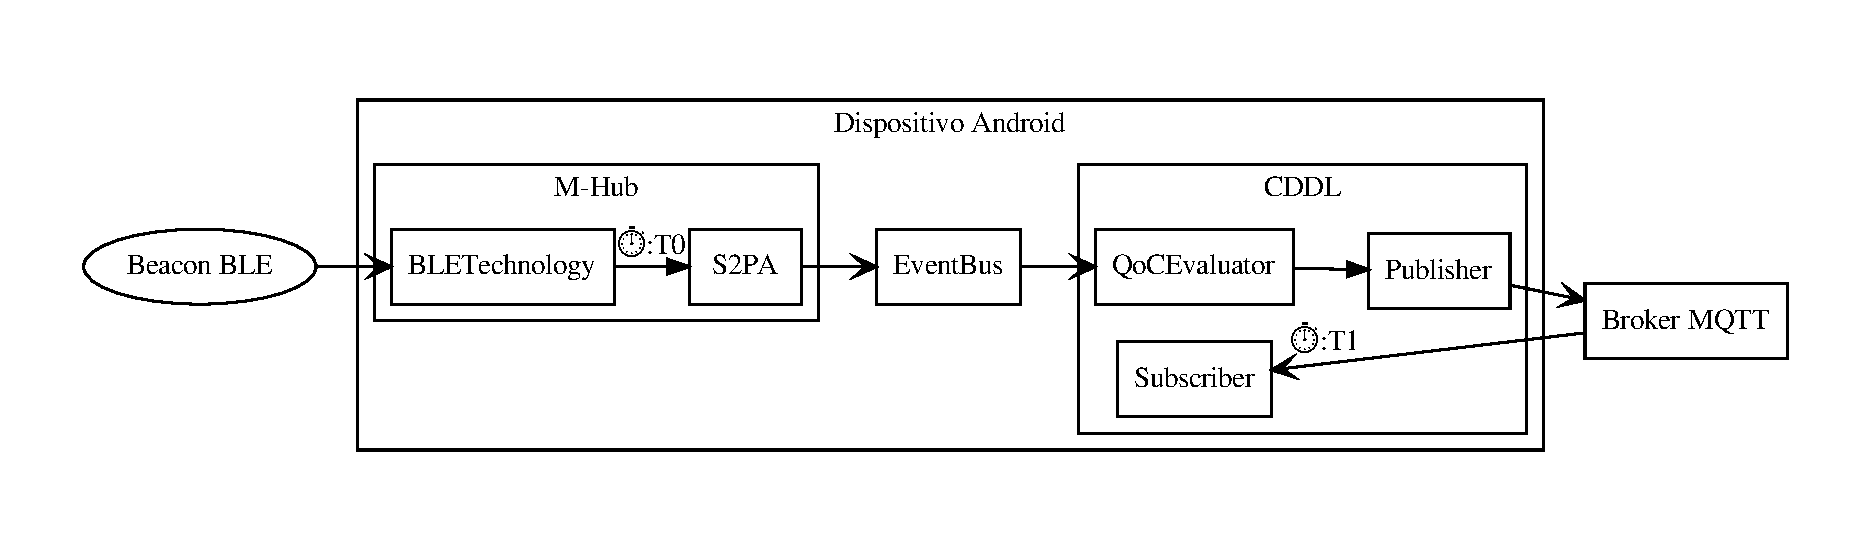
\includegraphics[width=0.95\linewidth]{img/performance-annotation}
		\fonte{\autoriapropria}

	\end{center}
	
\end{figure}

Para avaliar o percentual de perdas das notificações de eventos, é realizada uma comparação entre a quantidade de eventos de descoberta \smartobjs que foram gerados e quantas notificações foram entregues à aplicação, e será calculada através da \autoref{equ:acuracy}.
\begin{equation}
	\label{equ:acuracy}
	P_{perda} = \frac{EventosGerados - EventosNotificados}{EventosGerados} \cdot 100
\end{equation}

Onde $EventosGerados$ e $EventosNotificados$ se referem à quantidade de eventos gerados no \stwopa e à quantidade de notificações desses eventos que chegaram à aplicação, respectivamente.


\subsection{Cenário}\label{sub:cenario}
Para medir os parâmetros anteriores, foi desenvolvido um cenário de uso, onde será possível determinar tais aspectos.

Este cenário de uso consiste em uma casa onde cada cômodo é equipado com um \beacon \ble, calibrado de forma que o sinal emitido não possa ser detectado fora do cômodo e configurado para emitir 10 anúncios por segundo.
Uma pessoa portando um \smartphone é instruída a conduzir as atividades do dia a dia nesta residência.
Este \smartphone executa uma aplicação desenvolvida com o \middleware \mhubcddl que detecta os anúncios dos \beacons, determinando em qual região da casa o indivíduo se encontra.

Ao entrar em um cômodo, o \beacon será encontrado pelo \mhubcddl, gerando um evento de descoberta no \stwopa que deverá ser propagado para a aplicação.

\subsection{Simulação da locomoção na residência}\label{subsec:simulacao-loc}

A locomoção de um indivíduo em uma residencia como descrito na \autoref{sub:cenario} foi simulado utilizando um \dataset.
Os dados utilizados para a simulação deste experimento foram obtidos do \dataset disponibilizado por \citeonline{byrne:et-al:2018}\footnote{O \dataset pode ser obtido em \cite{byrne:kozlowski:dataset:2019}}.
Neste trabalho os autores instruíram que participantes conduzissem suas rotinas diárias em casa, enquanto sua localização na residência era monitorada.

O chão dos cômodos das casas foi marcado com etiquetas, onde cada etiqueta é uma imagem binária que codifica um número inteiro, e este, único para cada uma das etiquetas. Os participantes são equipados com uma câmera na região do torso que aponta em direção ao chão, detectando e interpretando qual etiqueta está visível no momento, e deste modo, identificando em qual cômodo o participante se encontra.

No trabalho citado, o autor realizou o experimento em 4 residências distintas, e estas foram denotadas de ``\texttt{Residence A}'', ``\texttt{Residence B}'', ``\texttt{Residence C}'' e ``\texttt{Residence D}''. Para cada residência, o experimento foi conduzido múltiplas vezes, e cada um denominado de ``\texttt{living\_1}'', ``\texttt{living\_2}'', ``\texttt{living\_3}'', \dots{}, ``\texttt{living\_n}''.


A fim de maximizar a quantidade de eventos de descoberta gerados na simulação, foi utilizado os dados do experimento ``\texttt{living\_2}'' da casa ``\texttt{Residence D}'' pois este experimento possui um dos maiores tempos de monitoramento e quantidade de entrada em cômodos em todo o \dataset. Os dados deste experimento consistem de 58 minutos de monitoramento de um indivíduo em uma casa de 10 cômodos. Os dados possuem uma resolução média de aproximadamente 11 medições por segundo.

Informações referentes à distribuição da quantidade de vezes em que o indivíduo visita um quarto estão sumarizadas na \autoref{fig:dataset-histogram}.

\begin{figure}[htb]
	
	\begin{center}
		
		\caption{\label{fig:dataset-histogram}Frequência de entrada por cômodo}
		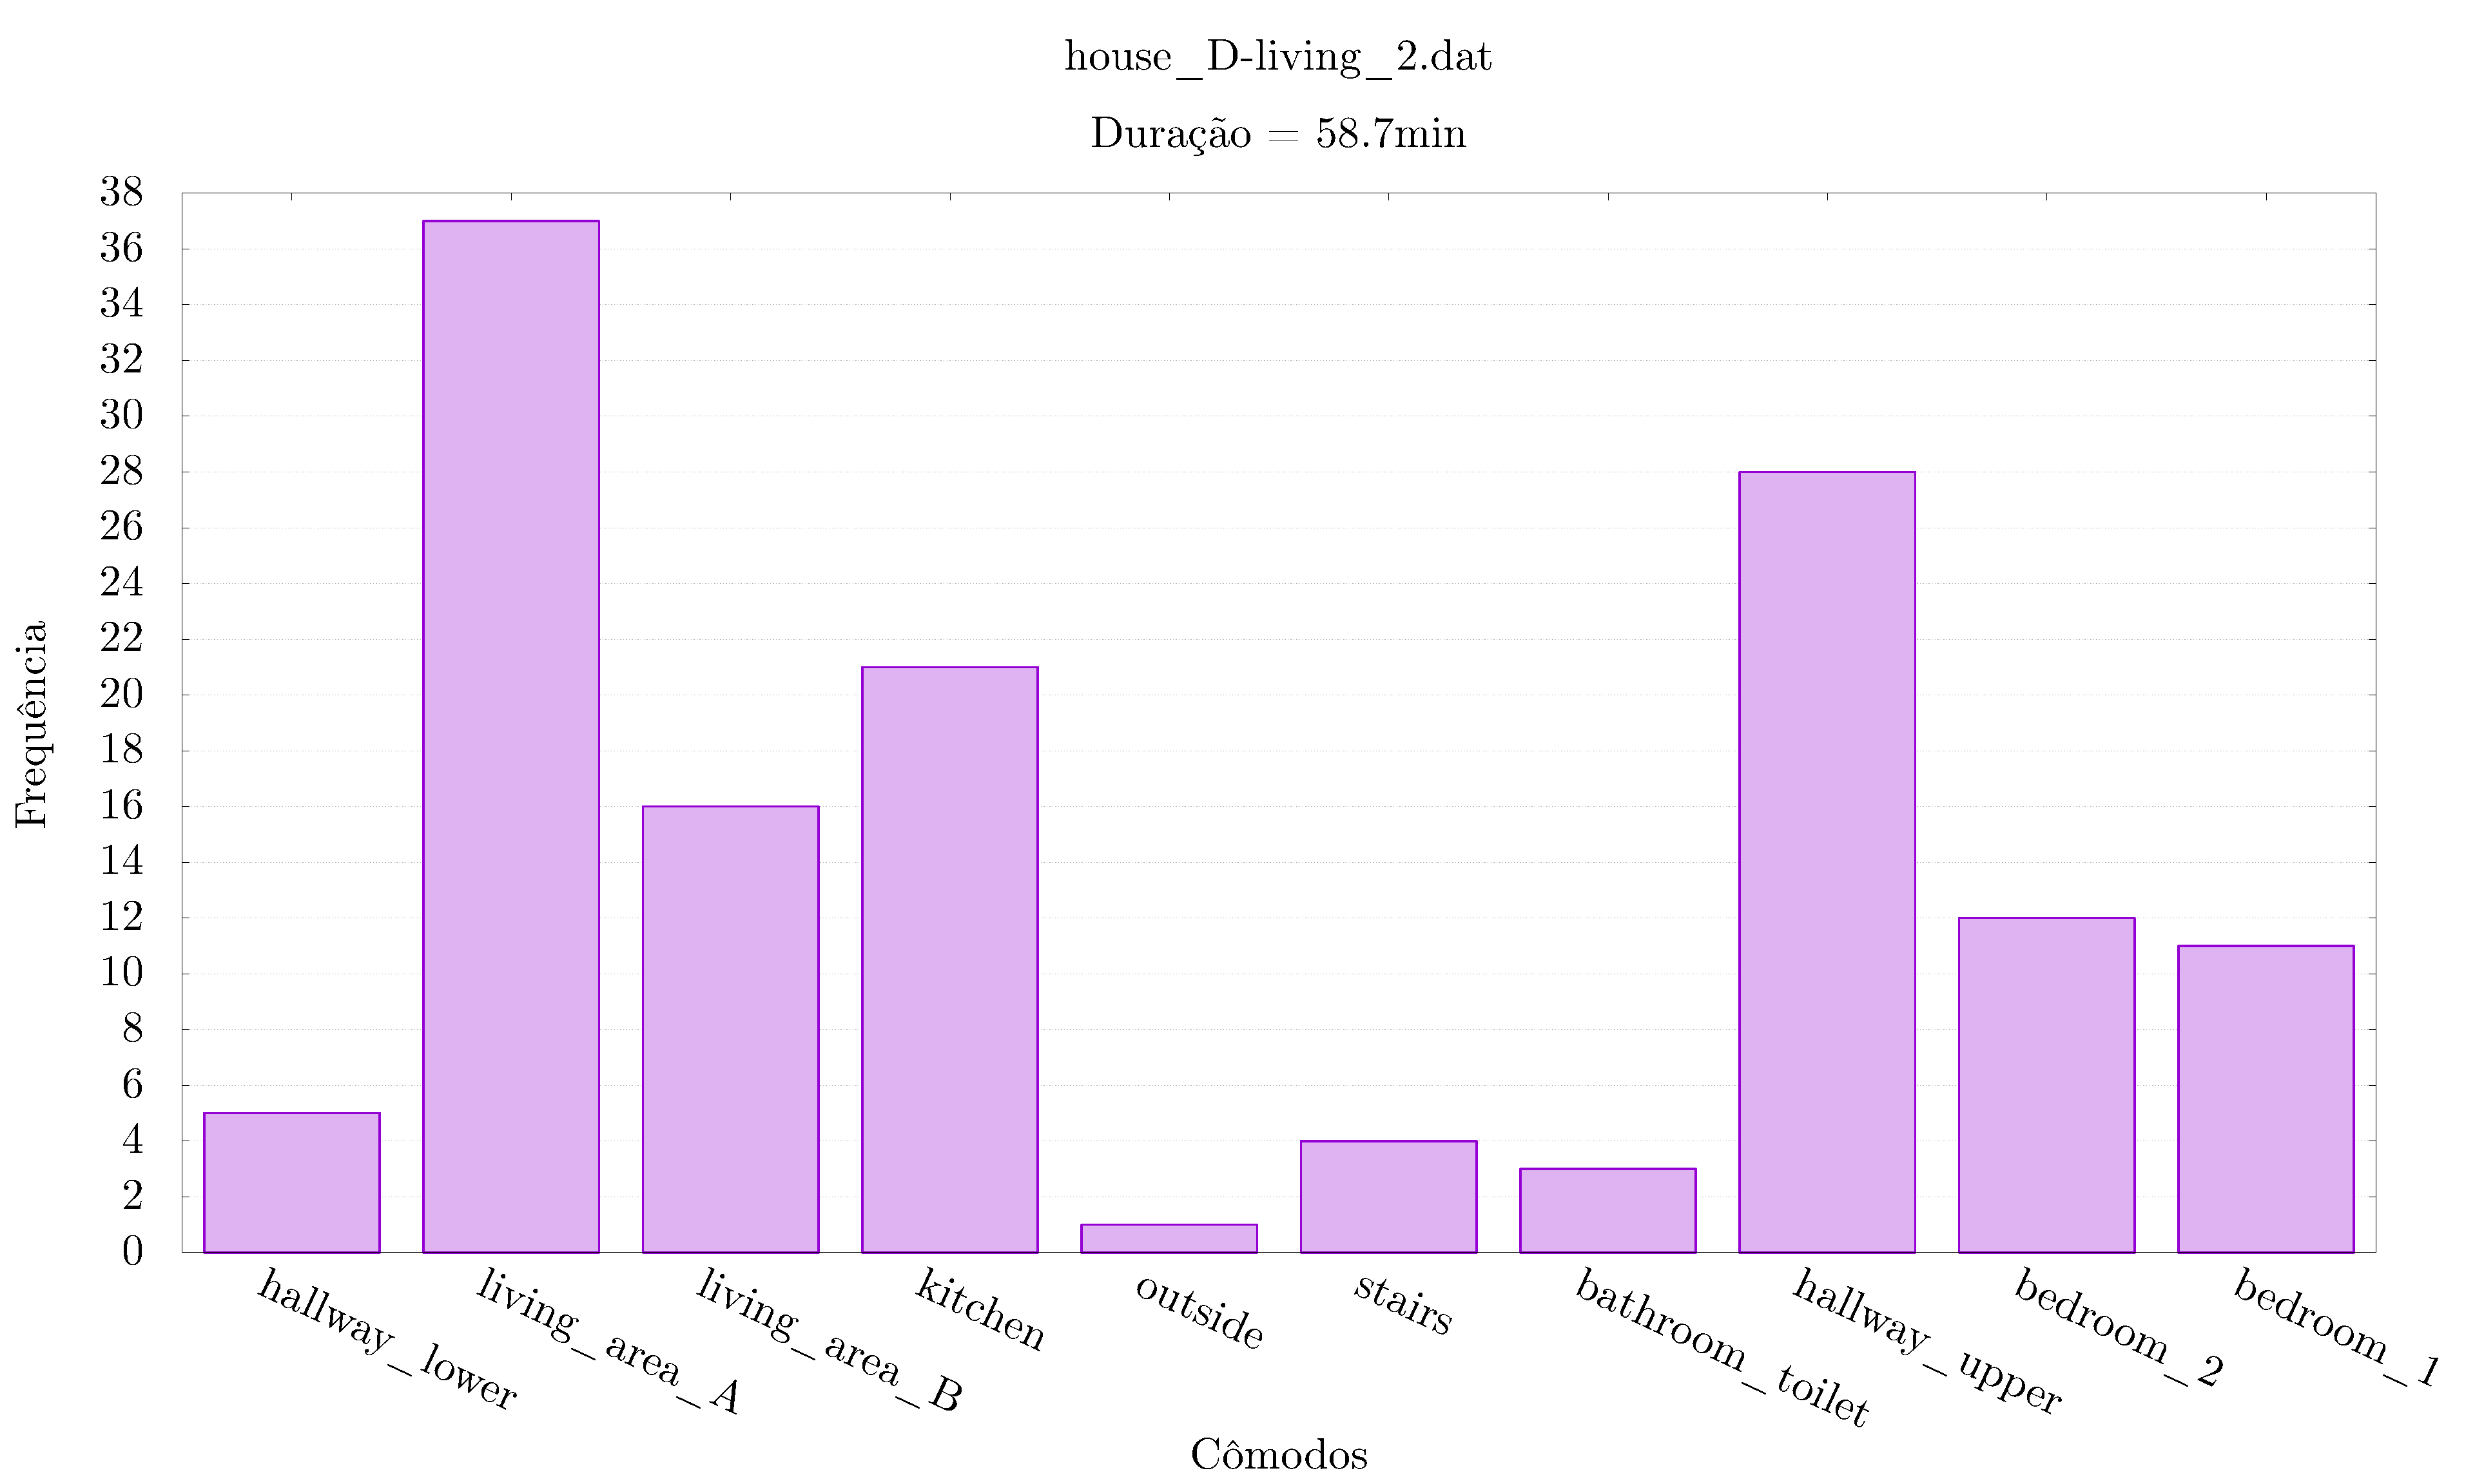
\includegraphics[width=0.95\linewidth]{img/dataset-histogram}
		\fonte{\autoriapropria}
		
	\end{center}

\end{figure}

O \dataset original é composto principalmente por um arquivo de texto que contém em cada linha uma representação de um momento no decorrer do experimento. Entre os dados contidos por linha, destaca-se o \timestamp da medição e a etiqueta detectada naquele instante. 

Realizou-se um pré-processamento no \dataset de forma a facilitar a utilização dos dados para fim da simulação, gerando um arquivo contendo 3 valores separadas por espaço em que cada linha representa o instante em que o participante entrou e permaneceu continuamente em um cômodo. Os 3 valores são: um identificador numérico do cômodo, o nome do cômodo e o \timestamp em que o indivíduo entrou naquele cômodo, como pode ser visto no \autoref{lst:preprocessed-dataset}.
\begin{lstlisting}[float=htb, language=python, caption={Parte do \dataset pré-processado}, label=lst:preprocessed-dataset]
#room    room-name          timestamp(seconds)
2        living_area_A      485.352
1        hallway_lower      506.273
6        stairs             513.380
8        hallway_upper      519.319
10       bedroom_1          526.159
8        hallway_upper      561.328
7        bathroom_toilet    565.832
8        hallway_upper      628.495
9        bedroom_2          632.065
\end{lstlisting}
	
\subsection{Simulação dos \beacons}

Como descrito anteriormente, o cenário consiste em um \beacon em cada cômodo de uma casa.
Utilizando os dados descritos na \autoref{subsec:simulacao-loc} foi realizado uma simulação de uma pessoa portando um \smartphone com uma aplicação \mhubcddl que detecta a presença de \beacons em cada cômodo onde o indivíduo adentra, estes \beacons foram configurados de forma a emitir 10 anúncios por segundo.  
É esperado, então,  que o aplicativo detecte um anúncio a cada 0.1 segundo em que o participante permanece em um cômodo. 

Para este experimento, cada anúncio detectado corresponde a um evento de descoberta gerado pelo \stwopa, este evento deve então ser propagado até a aplicação.

Utilizando o \dataset já descrito, a cada momento em que o participante entra em determinado cômodo, calcula-se a quantidade de anúncios o \beacon daquele cômodo transmitirá durante o tempo de permanência no local, o cálculo é apresentado a seguir.

\begin{equation}
	anuncios = \frac{tempoPermanencia}{0.1} 
\end{equation}


Onde $tempoPermanencia$ denota o tempo que o indivíduo permaneceu no cômodo.
Com isso foi possível calcular previamente os valores da \autoref{tab:generated-events-1}.  
Esta tabela mostra os valores do termo $EventosGerados$ na \autoref{equ:acuracy}, estes valores serão posteriormente comparados com a quantidade de eventos notificados para calcular o percentual de perdas.

\begin{table}[htb]
	\begin{center}
		\IBGEtab{
			\caption{Quantidade de eventos que serão gerados no experimento 1}
			\label{tab:generated-events-1}
		}{
			\begin{tabular}{lc}
				\toprule
				                               & $EventosGerados$ \\
				\midrule 
				\textbf{Eventos de descoberta} & 34814            \\
				\textbf{Eventos de conexão}    & 0                \\
				\textbf{Eventos de desconexão} & 0                \\
				\bottomrule
			\end{tabular}
		}{
			\fonte{\autoriapropria}
		}
	\end{center}
\end{table}



\subsection{Recursos computacionais}

O experimento descrito foi executado em um \smartphone Lenovo Moto Z Play, com processador de 8 núcleos e 2GHz, e 3GB de memória RAM.

\subsection{Resultados}

\newcommand{\nullval}{\textbf{---}}

\begin{table}[htb]
	\begin{center}
		\IBGEtab{
			\caption{Quantidade de eventos notificados no experimento 1}
			\label{tab:generated-events-1-results}
		}{
			\begin{tabular}{lccc}
				\toprule
							       & $EventosGerados$ & $EventosNotificados$ & $P_{perdas}$ (\%) \\
				\midrule
				\textbf{Eventos de descoberta} & 34814            & 34814                & 0		     \\
				\textbf{Eventos de conexão}    & 0                & 0                    & \nullval	     \\
				\textbf{Eventos de desconexão} & 0                & 0                    & \nullval          \\
				\bottomrule
			\end{tabular}
		}{
			\fonte{\autoriapropria}
		}
	\end{center}
\end{table}

\begin{table}[htb]
	\begin{center}
		\IBGEtab{
			\caption{Performance da entrega de mensagens do experimento 1}
			\label{tab:experiment-1-performance}
		}{
			\begin{tabular}{lccccc}
				\toprule
				                                           & Média & Desvio padrão & Mínimo & Máximo & Intervalo de 95\% de confiança \\
				\midrule
				$\bm{\Delta t_{descoberta}}$ \textbf{(ms)} & 20.1  & 3.7           & 7.0 & 78.9 & 20.1 $\pm$ 0.03 	              \\
				\bottomrule
			\end{tabular}
		}{
			\fonte{\autoriapropria}
		}
	\end{center}
\end{table}

\subsection{Análise dos resultados}

Mesmo com os \beacons configurados para realizarem \broadcast a cada 0.1 segundo, o que representa uma frequência muito alta para aplicações similares---como exemplo, em \citeonline{kim:et-al:2016} o autor utiliza 1 broadcast a cada dois segundos---a solução conseguiu notificar a aplicação em um tempo na casa de milissegundos.  
Este tempo pode ser considerado é desprezível para aplicações reais.

Do ponto de vista do percentual de perdas, a pesar de um grande número de eventos em um curto espaço de tempo, não houve perdas de notificações de eventos de descobertas dos \beacons.

A solução apresenta características satisfatórias para o uso em aplicações onde as interações com \smartobjs não são baseadas em conexões, como é o caso de aplicações de localização \textit{indoor}.

\section{Experimento 2}

O segundo experimento visa avaliar o desempenho e o percentual de perdas da solução proposta, entretanto levando em consideração também os eventos de conexão que não foram analisados no primeiro experimento.

\subsection{Métricas}

As avaliações de desempenho e percentual de perdas deste experimento são agora baseadas no tempo entre eventos de \emph{descoberta} no \stwopa e notificações de \emph{conexão} na aplicação.  
A \autoref{equ:performance-ready} será utilizada para avaliar a performance da solução.
\begin{align}
	\label{equ:performance-ready}
	\Delta t_{conectado} &= t_{conexao,app} - t_{descoberta,\stwopa}
\end{align}

Onde $t_{descoberta,\stwopa}$ é o \timestamp de quando um evento de descoberta de um \smartobj é gerado no \stwopa, $t_{conexao,app}$ é \timestamp de quando o a notificação do evento de conexão do mesmo \smartobj é entregue a aplicação e $\Delta t_{conectado}$ o tempo que processo de descoberta até notificação de conexão levou para ser concluído.

Neste contexto, será medido o tempo entre o evento de \emph{descoberta} do \smartobj no \stwopa e a notificação do evento de \emph{conexão} na camada de aplicação.
Deseja-se saber em quanto tempo desde a descoberta do dispositivo os dados disponibilizados estarão disponíveis para o consumo pela aplicação.

Para medir o percentual de perdas será utilizado a \autoref{equ:acuracy}.

\subsection{Cenário}

O experimento consiste em um cenário de uso composto por uma casa equipada com um sistema multimídia na sala de estar que possibilita que \smartphones se conectem a ele através de \bluetooth, onde o conteúdo da televisão se adapta de acordo com os usuários que estão presentes na sala, e a interação com as aplicações da televisão digital acontece através do \smartphone.

O sistema multimídia pode ter ciência de qual usuário está presente através dos \smartphones conectados no momento, pois ele armazena a relação dos moradores da residência com seus respectivos \smartphones.


Uma aplicação \android foi desenvolvida com o \middleware \mhubcddl que permanece ativamente procurando e se conectando ao sistema multimídia no ambiente. Ao entrar na sala de estar o sistema multimídia é encontrado e em seguida a conexão é estabelecida. Quando o usuário sai da sala de estar a conexão é desfeita. 

%-------------------------------------


\subsection{Simulação do sistema multimídia}

Para este experimento foi feita uma simulação de um indivíduo se locomovendo em uma residência. Foram utilizados os dados do \dataset descrito na \autoref{subsec:simulacao-loc} para esta simulação.

Escolheu-se também o experimento ``\texttt{living\_2}'' da casa ``\texttt{Residence D}'' por fornecer um dos maiores tempos de monitoramento do participante juntamente com a maior quantidade de visitas à sala de estar. Será utilizado apenas a parte do \dataset referentes à entradas no cômodo denotado como ``\texttt{living\_area\_A}'' na \autoref{fig:dataset-histogram}, pois este cômodo foi escolhido como a sala de estar onde o sistema multimídia se localiza.

Desta forma, a todo momento em que o participante entra na sala de estar acontece interações entre o aplicativo e o sistema multimídia, essas interações são compostas de um evento de descoberta, seguido por um evento de conexão.
Ao sair do quarto um evento de desconexão é também gerado. Cada um desses eventos são gerados pelo \stwopa e notificados posteriormente à aplicação.

Como pode ser notado na \autoref{fig:dataset-histogram}, é possível determinar a quantidade de vezes em que o participante entra na sala de estar.
Deste modo pode-se saber a quantidade total de interações com o sistema multimídia ocorrerão de antemão.
A \autoref{tab:generated-events-2} sumariza os resultados esperados para o experimento.

\begin{table}[htb]
	\begin{center}
		\IBGEtab{
			\caption{Quantidade de eventos que serão gerados no experimento 2}
			\label{tab:generated-events-2}
		}{
			\begin{tabular}{lc}
				\toprule
				                               & $EventosGerados$ \\
				\midrule 
				\textbf{Eventos de descoberta} & 37               \\
				\textbf{Eventos de conexão}    & 37               \\
				\textbf{Eventos de desconexão} & 37               \\
				\bottomrule
			\end{tabular}
		}{
			\fonte{\autoriapropria}
		}
	\end{center}
\end{table}

Para a modelagem do tempo entre a descoberta e conexão do \smartphone e o \smartobj, foram utilizados dados empíricos coletados pelo autor.
Um \smartobj baseado na plataforma Arduino e com suporte à tecnologia \ble foi construído, e várias amostras de tempo entre a descoberta deste dispositivo e a conexão com ele foram tomadas.

\subsection{Resultados}

\vphantom{abc}

\begin{table}[ht]
	\begin{center}
		\IBGEtab{
			\caption{Quantidade de eventos notificados no experimento 2}
			\label{tab:generated-events-2-results}
		}{
			\begin{tabular}{lccc}
				\toprule
							       & $EventosGerados$ & $EventosNotificados$ & $P_{perdas}$ (\%) \\
				\midrule
				\textbf{Eventos de descoberta} & 37               & 37                   & 0		     \\
				\textbf{Eventos de conexão}    & 37	          & 37                   & 0		     \\
				\textbf{Eventos de desconexão} & 37	          & 37                   & 0	             \\
				\bottomrule
			\end{tabular}
		}{
			\fonte{\autoriapropria}
		}
	\end{center}
\end{table}

\begin{table}[ht]
	\begin{center}
		\IBGEtab{
			\caption{Performance da entrega de mensagens do experimento 2}
			\label{tab:experiment-2-performance}
		}{
			\begin{tabular}{lccccc}
				\toprule
				                          & Média & Desvio padrão & Mínimo & Máximo & Intervalo de 95\% de confiança \\
				\midrule
				$\bm{\Delta t_{conectado}}$ \textbf{(ms)} & 501.4 & 60.8         &425.1        & 654.5       &	501.4 $\pm$ 19.6	                  \\
				\bottomrule
			\end{tabular}
		}{
			\fonte{\autoriapropria}
		}
	\end{center}
\end{table}

\subsection{Análise dos resultados}

Assim como no experimento 1, não foi possível observar perda de notificações neste experimento.
O tempo entre a descoberta de um \smartobj no ambiente e sua conexão, e consequentemente a disponibilidade de consumir os dados oferecidos por este, se manteve em torno de 500 milissegundos.

Isto implica que uma aplicação que necessite de dados oferecidos por sensores no ambiente, começaria a receber estes dados em média 0.5 segundo após o primeiro encontro com este dispositivo.

Tomando como exemplo o cenário em que uma aplicação faz uso de dados de umidade do ar fornecidos por sensores em postes públicos que se comunicam através da tecnologia \ble, é possível fazer uma análise de o quão rápido o usuário pode passar nas redondezas do sensor sem perder a oportunidade de capturar o dado.
Assumindo que o raio de cobertura do sinal \bluetooth é de 5 metros, e que o usuário tem que atravessar o diâmetro completo para perder o sinal, ele deve percorrer 10 metros desde o momento que encontra o dispositivo até perder o sinal.

Dividindo a distância que ele deve percorrer pelo tempo médio que uma conexão é realizada, temos:
\[
	\frac{10\si{\meter}}{0.5\si{\second}} = 20\si{m/s} = 72\si{km/h}
\]
A implicação deste valor é que o usuário pode se locomover pelo entorno do sensor com até 72\si{km/h}, e ainda assim adquirir o dado que a aplicação necessita. Fazendo com que o usuário não necessite diminuir a velocidade de seu trajeto estando a pé, de bicicleta ou conduzindo veículo motorizado na maioria dos cenários urbanos.

